\documentclass[12pt]{article}
\usepackage{amsmath}
\usepackage{graphicx}
\usepackage{float}
\usepackage{listings}
\usepackage{xcolor}

\begin{document}

\title{Desafío Final}
\author{Team Mustabot 2022}
\date{\today}

\maketitle
\section*{Desafío}
El robot tiene la misión de completar satisfactoriamente y en menos de 2 minutos el siguiente circuito:
%adjuntamos la imagen del circuito

para esto, deberá usar todos los sensores que posee.
Tendrán 1:30 minutos para programar el robot, durante ese tiempo pueden probarlo las veces que quieran, cuando entreguen el robot, tendrán 10 minutos para cargar las baterias
y hacer cambios en el código, los cuales se podrán subir al robot antes de la competencia, pero no podrán probarlo.
Luego de la primera ronda tendrán 30 minutos para implementar los cambios que el robot requieran para funcionar perfectamente, luego de eso,
será la ronda final.
la pista posee checkpoints, cuando el robot supere adecuadamente un checkpoint, se guardaran los puntos que el robot ha conseguido en ese tramo
El criterio de evaluación será el siguiente:
%creamos una lista con punteo
\begin{itemize}
    \item 50 puntos por cada checkpoint superado
    \item 10 puntos por cada checkpoint superado en menos de 1 min segundos
    \item 20 puntos por cada checkpoint superado en menos de 30 segundos
    \item 30 puntos por cada checkpoint superado en menos de 20 segundos
    \item 200 puntos por completar el circuito
\end{itemize}
%añadimos una imagen de la pista
\section*{Pista}
\begin{figure}[H]
    \centering
    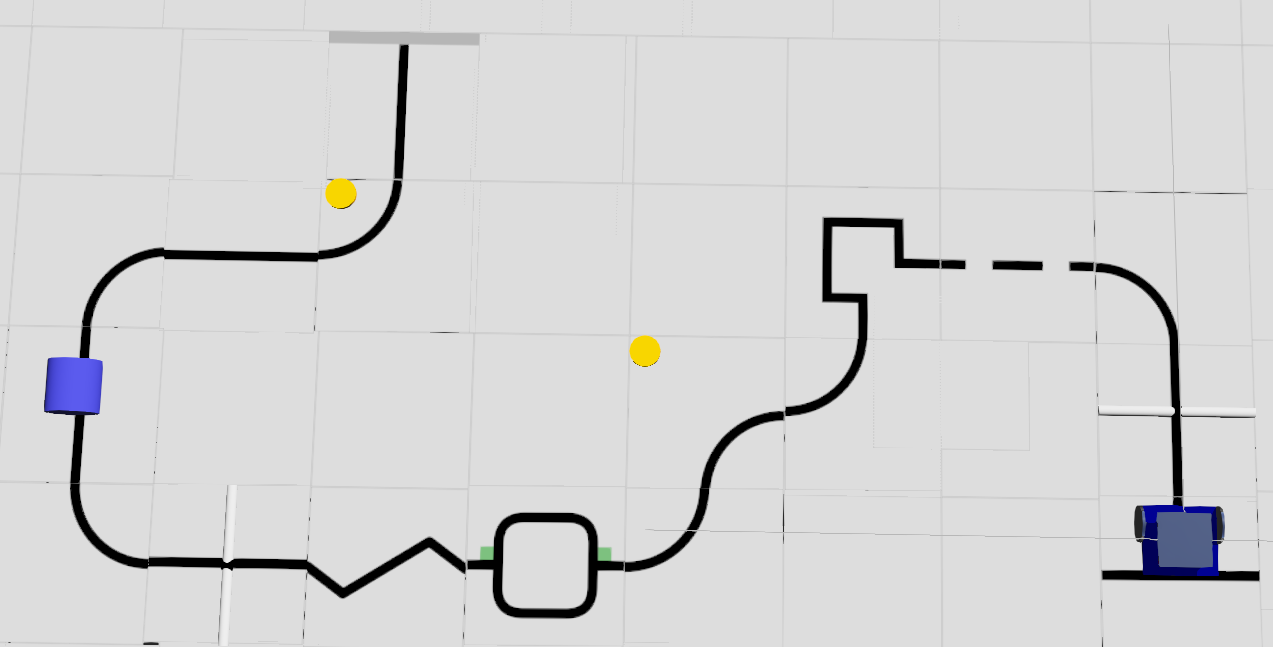
\includegraphics[width=1.25\textwidth]{simulacion_imagenes/pista_desafio_final.png}
    \caption{Pista}
    \label{fig:pista}
\end{figure}
\end{document}